\begin{frame}
  \frametitle{How to start TDD?}
  \pause
  \begin{itemize}
      \item Small project, at home\pause
      \item Big project, at work\pause
      \item Code coverage\pause
      \item bug report -> write test -> fix\pause
      \item new features -> TDD\pause
      \item write test -> refactor legacy code
  \end{itemize}
\end{frame}

\begin{frame}
  \frametitle{Conclusion}
  \begin{itemize}
      \item Quaility is form and function\pause
      \item Test suite -> improve form\pause
      \item Test suite -> lock function\pause
      \item TDD -> Test suite
  \end{itemize}
\end{frame}

\vspace*{-12.5mm}    
\begin{frame}[fragile, plain]
\frametitle{}
\hspace*{-11mm}
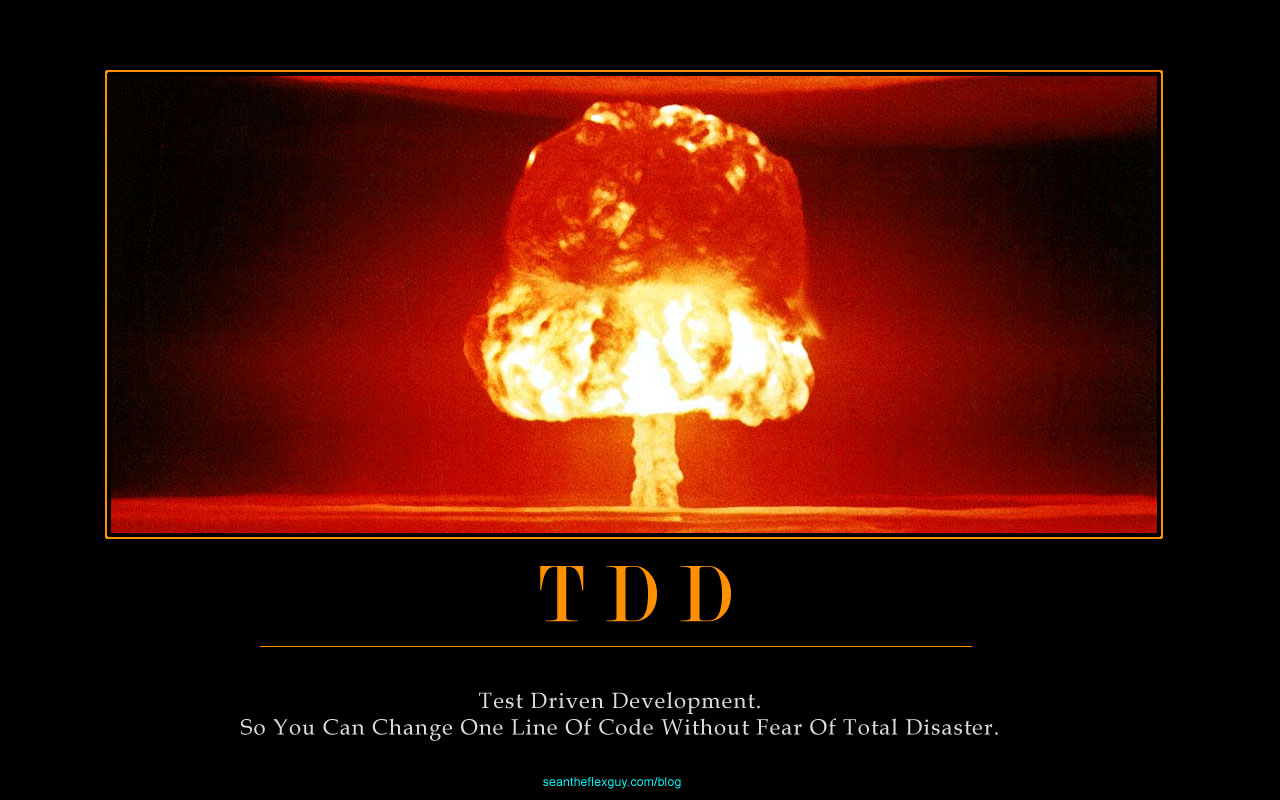
\includegraphics[width=\paperwidth, width=\paperwidth]{tdd.jpg}
\end{frame}

